\documentclass[11pt]{article}% uses letterpaper by default

%---------- Uncomment one of them ------------------------------
\usepackage[includeheadfoot, top=1in, bottom=1in, hmargin=1in]{geometry}

% \usepackage[a5paper, landscape, twocolumn, twoside,
%    left=2cm, hmarginratio=2:1, includemp, marginparwidth=43pt, 
%    bottom=1cm, foot=.7cm, includefoot, textheight=11cm, heightrounded,
%    columnsep=1cm, dvips,  verbose]{geometry}
%---------------------------------------------------------------
\usepackage{fancyhdr}
\renewcommand{\footrulewidth}{0.4pt}% default is 0pt
\usepackage{verbatim}
\usepackage{url}
\usepackage{cancel}
\pagestyle{fancy}
\usepackage{graphicx}
\usepackage{setspace}
\singlespacing
%\doublespacing
%\onehalfspacing
\usepackage{varwidth}

\newcommand{\degrees}{\ensuremath{^\circ}}
\newcommand{\arcmin}{\ensuremath{'}}
\newcommand{\arcsec}{\ensuremath{"}}
\newcommand{\hours}{\ensuremath{^\mathrm{h}}}
\newcommand{\minutes}{\ensuremath{^\mathrm{m}}}
\newcommand{\seconds}{\ensuremath{^\mathrm{s}}}

\newcommand{\s}[0]{\phantom{i}} %sets up \s command
\newcommand{\m}[0]{\phantom{abcde}} %sets up \m command
\providecommand{\e}[1]{\ensuremath{\times 10^{#1}}} %sets up \e command
\setlength{\parindent}{0.2in} %new paragraph indent
\usepackage{indentfirst} % indent the first paragraph of a section
\usepackage{amsmath,amssymb}
\usepackage{enumitem}

\lhead{Astronomy Lab II}
\rhead{Spring 2022}
\lfoot{Mead}
\rfoot{Mon 6-9pm}
\cfoot{\thepage}

%\newcommand{\exercisename}{7}
\begin{document}

\begin{center}
\huge{Lab 6: Dark Matter}\\ \medskip \Large{February 28, 2022}
\end{center}

%%%%%%%%%%%%%%%%%%%%%%% INTRODUCTION %%%%%%%%%%%%%%%%%%%%%%%
\section{Introduction}
% Note to future readers of this tex doc - we brought in a speaker from the Columbia XENON experiment to give an introduction to DM and DM detection experiments.  The students also received a tour of the XENON lab.
\noindent
We have just learned about \textit{dark matter} and about the search for the elusive ``missing mass" in our Universe.  In this portion of the lab, you will dive a little deeper into the some of the evidence for dark matter, known as \textit{rotation curves}.

\medskip \noindent
The rotation curve of a galaxy is a measurement of how fast the galaxy rotates as a function of distance from the center.  Galaxies don't rotate as solid bodies (like records on a turntable or merry-go-rounds); rather, they rotate \textit{differentially}, with the inner parts moving faster than the outer parts. You will use Newton's laws to investigate this differential rotation and learn how we can use the rotation curve to determine if dark matter is really a solution to the mystery of the ``missing mass".

%%%%%%%%%%%%%%%%%%%%%%% SOLAR SYSTEM %%%%%%%%%%%%%%%%%%%%%%%
\section{Differential Rotation in the Solar System}
\noindent
In space, almost everything is orbiting something: the moon orbits Earth, Earth orbits the Sun, the Sun orbits the center of the Milky Way galaxy, etc. All of this motion is due (we suspect) to the force of gravity:

\begin{equation}
F = \frac{G M_1 M_2}{r^2}
\end{equation}

\noindent Masses $M_1$ and $M_2$ actually both orbit their common \textit{barycenter}, or center of mass. When more complicated mass distributions are involved (e.g., many orbiting bodies, as in the Solar System or the Milky Way), each mass is subject to the gravitational force of all the mass within its own orbit: for example, the gravitational force on Earth is, properly:

\begin{equation}
F = \frac{G M_{\textrm{Earth}} \times (M_{\odot} + M_{\textrm{Mercury}} + M_{\textrm{Venus}})}{r^2}
\end{equation}

\noindent where $r$ is the distance between Earth and the center of mass of all four objects. However, the Sun is so much more massive than anything else in the Solar System that we can ignore the contribution of the other planets and write:

\begin{equation}
F = \frac{G M_{\textrm{Earth}} \times M_{\odot}}{r^2}
\end{equation}

\noindent where $r$ is the distance between the Earth and the Sun. More generally, we can write:

\begin{equation} \label{eq:grav}
F = \frac{G M_{\textrm{planet}} \times M_{\textrm{star}}}{r^2}
\end{equation}


\noindent In our Solar System, the planets move on very nearly circular orbits. The force on an object on a circular orbit is described by the equation:

\begin{equation} \label{eq:CF}
F = \frac{M v^2}{r}
\end{equation}

\noindent where $M$ is the orbiting body's mass, $v$ is its velocity, and $r$ is the radius of its orbit. (This is the formula for \textit{centripetal force}.) If we are right, and the force of gravity is really what is making the planets orbit the Sun, then a little bit of algebra will tell us how the velocity of a planet is related to its distance from the Sun.  \textbf{Do the following in your lab notebook:}

\begin{enumerate}
    \item The force of gravity on an orbiting body must balance its centripetal force. Consider a planet ($M_{\textrm{planet}}$) orbiting the Sun. Set equations \ref{eq:grav} and \ref{eq:CF} equal to each other and solve for $v$ in terms of $M_{\odot}$, $G$, and $r$.
    \item Now we have a theoretical prediction for the velocity of the orbits of the planets. Using information from Table \ref{tab:planets}, calculate the orbital velocity of each planet (as predicted by the equation you just derived) in \textbf{km/s} and record it in your notebook, making two columns: one for the planet's name, and one for their respective calculated orbital velocity. Make sure to keep track of your units and be sure they match!
    \item Using these values, plot the theoretical rotation curve (in km/s vs. AU) for our Solar System. Use either graph paper or a spreadsheet of your choice.
    \item Using the measured values in Table \ref{tab:Solar_system}, plot the actual rotation curve (in km/s vs. AU). (Don't forget to label the axes and indicate which plotted curve is which!). Do you think gravity is responsible for the orbits of the planets?
\end{enumerate}

\begin{table}[h!]
    \centering
    \begin{tabular}{cccccc}
        \hline
        \hline
         Planet & Semimajor & Orbital & Sidereal Orbital & Average Orbital & Your Calculated \\
          &  axis (AU) & Eccentricity & Period (yr) & Velocity (km/s) & Velocity (km/s) \\
        \hline
        Mercury & 0.3871 & 0.2056 & 0.2408 & 47.9150 & \\
        Venus   & 0.7233 & 0.0068 & 0.6152 & 35.0435 & \\
        Earth   & 1.0000 & 0.0167 & 1.0000 & 29.8061 & \\
        Mars    & 1.5237 & 0.0934 & 1.8809 & 24.1456 & \\
        Jupiter & 5.2028 & 0.0483 & 11.8622 & 13.0730 & \\
        Saturn  & 9.5388 & 0.0560 & 29.4577 & 9.65161 & \\
        Uranus  & 19.1914 & 0.0461 & 84.0139 & 6.80864 & \\
        Neptune & 30.0611 & 0.0097 & 164.793 & 5.43715 & \\
    \end{tabular}
    \caption{Solar System Data}
    \label{tab:Solar_system}
\end{table}


%%%%%%%%%%%%%%%%%%%%%%% ROTATION CURVES %%%%%%%%%%%%%%%%%%%%%%%
\break
\section{Differential Rotation in a Galaxy}

\noindent
In the last part, we used our knowledge of the mass of the Sun to predict the orbital velocity of the planets. For galaxies, we have to work backwards -- we don't know the mass of a galaxy, but we can use the orbits of the stars around the center to deduce what the galaxy's mass must be. Figure 1 shows a measured rotation curve for the galaxy NGC 2742. The positive values of radial velocity are for the stars moving away from us, while the negative velocities are for stars moving towards us. Negative radius values are just used to indicate an opposite side of the galaxy from the positive radius values. 

\begin{figure}[h!]
\center
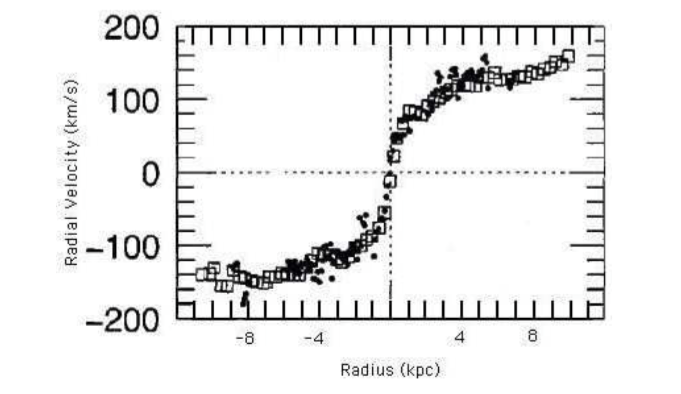
\includegraphics[scale=0.6]{Images/rotation_curve.png}
\caption{The rotation curve of NGC 2742.}
\label{rotcurve}
\end{figure}

\begin{enumerate}
\item Draw a table in your notebook with 5 columns: \textit{Radius (kpc)}, \textit{Rotational Velocity (km/s)}, \textit{Gravitational Mass ($M_{\odot}$)}, \textit{Luminosity ($L_{\odot}$)}, and \textit{Luminous Mass ($M_{\odot}$)}.
Select 7 evenly spaced radii from Figure \ref{rotcurve}, either all positive or all negative, and record them in your table.
\item Use Figure \ref{rotcurve} to measure the radial velocity at each of your radii. Record them in your table.
\item Use the equation you derived in section 2, question 1 to solve for enclosed mass $M$ as a function of velocity $v$, orbital radius $r$, and the constant $G$. (\textit{Hint}: Recall that the mass in the equation you derived above was $M_\odot$ because the Sun's mass dominates our Solar System, but really, the mass that should be used is the total mass contained \textit{within} the orbit.)
\item Solve for the amount of galactic mass within each of the radii you chose. Record these (very big) values in the table, under ``gravitational mass" (since this is mass predicted by gravity). Pay attention to units!
\end{enumerate}

\noindent
Now you have weighed the galaxy and can see that gravity predicts a mass equal to billions and billions of stars.  We can compare this to the amount of light from the galaxy, since the light comes from the stars and gas it contains.  Figure 2 shows the amount of galactic light that comes from within different radii. 

\medskip \noindent
The comparison we're going to make is easier for some galaxies than others. It is harder to figure out how much light is coming from a galaxy the more ``edge-on'' it is, because if we are looking at the side of the galaxy, a lot of the light is blocked by dust. 
In contrast, when we look at a galaxy ``face-on,'' we see almost all of its light, but it is harder to accurately determine the galaxy's rotational velocity (because most of the rotational velocity is perpendicular to our line of sight).


\begin{figure}[h!]
\center
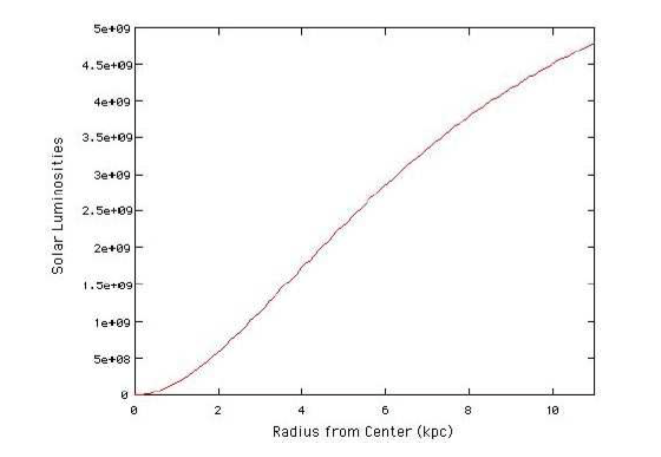
\includegraphics[scale=0.6]{Images/enclosed_luminosity.png}
\caption{The amount of light emitted from inside a given radius in NGC 2742.}
\label{luminosity}
\end{figure}

\begin{enumerate}[resume]
%\setcounter{enumi}{4}
\item At the radii that you have chosen, determine a value for the luminosity of the galaxy and record it in the table. (The ``e''s in the luminosity values are powers of ten: ``2e+09" means $2 \e{9}$).
\item Now calculate how much mass must be present in the galaxy based on how much light we see. Assume that it takes roughly two solar masses of matter to produce one solar luminosity. (This is based on how many low mass and high mass stars we think are typically in a galaxy.) Record the values in the table under \textit{Luminous mass}. 
\item Plot each of the masses (gravitational and luminous) versus radius, remembering to label your axes.
\item Determine the \textit{mass-to-light ratio} for NGC 2742 at your largest radius (within the entire galaxy) by dividing your gravitational mass by your luminous mass. 
\item What can you conclude about the matter in NGC 2742? 
In other words, what percentage of the total mass is luminous? 
What percent cannot be accounted for by the light that we see?
Why is this so-called ``dark matter'' termed ``dark?''
\end{enumerate}

%%%%%%%%%%%%%%%%%%%%%%% CONCLUSIONS %%%%%%%%%%%%%%%%%%%%%%%
\section{Conclusions}
\begin{enumerate}

\item What is one thing you learned about direct detection dark matter experiments?
\item Based on the above, are you convinced dark matter exists?
\item Figure 3 shows two galaxies that we cannot use to search for dark matter. Why not?
\item Vera Rubin work on galaxy rotation curves and identified the very problem you worked on in this lab, providing the very first evidence for dark matter.  Read up on Vera Rubin and write a short paragraph on something interesting you found about her life or work as a pioneering female astronomer. \url{https://en.wikipedia.org/wiki/Vera_Rubin}
\item What is one lingering question you have after this lab?
\item If the lab was perfectly clear to you, what did you like or dislike? If not, what confused you? Any other feedback?
\end{enumerate}

\begin{figure}[t!]
\center
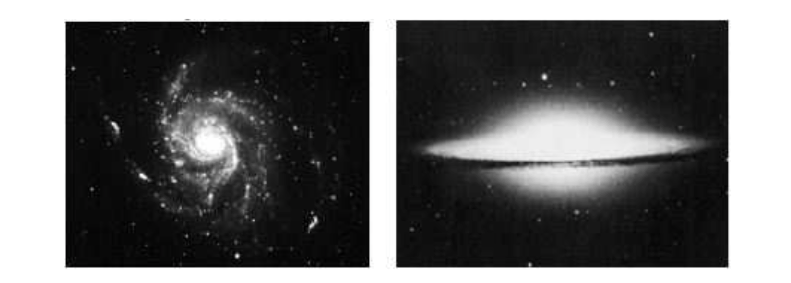
\includegraphics[scale=0.6]{Images/galaxies.png}
\caption{Left: M101, the Pinwheel Galaxy. Right: M104, the Sombrero Galaxy.}
\label{galaxies}
\end{figure}

\end{document}

